\documentclass{scrartcl}
\usepackage[utf8]{inputenc}
\usepackage{hyperref}
\usepackage{url}
\usepackage{natbib}
\usepackage{graphicx}
\usepackage{float}
\usepackage{listings}
\usepackage{xcolor}
\usepackage{cleveref} % this must be the last package to be loaded

\definecolor{codegreen}{RGB}{193, 193, 193}
\definecolor{codegray}{RGB}{193, 193, 193}
\definecolor{codepurple}{RGB}{193, 193, 193}
\definecolor{backcolour}{RGB}{21,21,21}
\definecolor{codecolor}{RGB}{193, 193, 193}

\lstdefinestyle{mystyle}{
    backgroundcolor=\color{backcolour},   
    commentstyle=\color{codegreen},
    keywordstyle=\color{magenta},
    numberstyle=\tiny\color{codegray},
    stringstyle=\color{codepurple},
    basicstyle=\ttfamily\footnotesize\color{codecolor},
    breakatwhitespace=false,         
    breaklines=false,                 
    captionpos=b,                    
    keepspaces=true,                               
    showspaces=false,                
    showstringspaces=false,
    showtabs=false,                  
    tabsize=2,
    frame=none
}

\lstset{style=mystyle} 
\lstset{
  framesep=3pt,
  frame=single
}

\newcommand{\emailaddr}[1]{\href{mailto:#1}{\texttt{#1}}}

\title{\LARGE
  MarafoNet, Marafone on the net
}
\subtitle{Final Report for the Distributed Systems Course 2025}

% Consider watching:
% https://www.youtube.com/watch?v=ihxSUsJB_14
% https://www.youtube.com/watch?v=XTFWaV55uDo

\author{
    Bagattoni Federico \\ \small{\emailaddr{federico.bagattoni@studio.unibo.it}}
    \and
    Jacopo Turchi \\ \small{\emailaddr{jacopo.turchi@studio.unibo.it}}
}

\date{\today}

\begin{document}

\maketitle

\begin{abstract}
    Up to $\sim$2000 characters briefly describing the project. PROVA PER CAPIRE SE COMPILA PER BENE.
\end{abstract}

\section*{Disclaimer}

During the preparation of this work, the author(s) used GitHub Copilot and Google Gemini for debugging and prototyping purposes.

After using this tool/service, 
the author(s) reviewed and edited the content as needed 
and take(s) full responsibility for the content of the final report/artifact.

%\section*{Quick \LaTeX{} suggestions}
%
%If you need to cite a reference, you can use the \texttt{cite} command, 
%like providing the BibTex key of some entry in the \texttt{references.bib} file, 
%.g.: \cite{adams1995hitchhiker}.
%
%You can find pre-coocked BibTex entries for most Computer Science papers on \href{https://dblp.uni-trier.de/}{DBLP}.
%
%If you need to include an image,
%let \LaTeX{} decide where to put it by using the \texttt{figure} environment,
%ith a \texttt{includegraphics} command inside it.
%
%If your need to reference a figure,
%se the \texttt{label} command to assign a label to the figure,
%and then use the \texttt{cref} command to reference it.
%
%Put figures in the \texttt{figures} folder.
%
%A complete example is shown in \cref{fig:universe}.
%
%\begin{figure}
%    \centering
%    \includegraphics[width=0.5\textwidth]{figures/universe.jpg}
%   \caption{This is an example image}
%    \label{fig:universe}
%\end{figure}
%
%Do \textbf{not} put any placement constraint on figures,
%such as \texttt{[h]} or \texttt{[h!]}.
%
%Same considerations apply for other floating elements 
%(e.g. tables, algorithms, listings, etc.).
%
%Do \textbf{not} use the \texttt{\textbackslash\textbackslash} or \texttt{\textbackslash newline} commands to break lines.
%
%Just leave an empty line between two paragraphs to start a new one.
%
%The new line will be automatically indented.
%
%This is intended: it is the \LaTeX{} way to separate capoverses.

\section{Concept}\label{concept}

\subsection*{Product Type}
This project is a web application accessible via a GUI.

\subsection*{Use Case}
The system digitalises the turn-based card game Marafone, applying the Emilia Romagna rules, to provide global accessibility. Users play via a web interface optimised for laptops, desktops, and tablets. The interaction model is turn-based, with players executing an action approximately every 30 seconds. System interaction requires account registration, but data storage is strictly limited to user credentials (username and password), with no additional information retained.

\subsection*{Need for Distribution}
Since the user base is concentrated in central Italy, geographical distribution is a secondary concern. However, a distributed architecture is required to:
\begin{itemize}
    \item Guarantee \textbf{data integrity} and robust state management across the system.
    \item Enable \textbf{parallel computation} for game logic and concurrent matches.
    \item Maintain \textbf{system stability and fault tolerance} under heavy load and in the case of node failures.
\end{itemize}

\section{Requirements elicitation and analysis}\label{requirements}

\subsection*{Glossary}
\begin{itemize}
  \item \textbf{Game:} A complete playing session that concludes with the win of a team.
  \item \textbf{Match:} A single round within a Game, starting with the dealing of cards and ending when players run out of cards.
  \item \textbf{Trump suit:} The dominant suit designated for the current Match, chosen by the first player. Cards of this suit outrank all cards of the other three suits.
  \item \textbf{Current Player:} The player who currently holds the right to execute an action (playing a card or choosing the Trump suit).
  \item \textbf{Trick:} A sequence where each player plays exactly one card. The Trick is won by the player who played the highest value card of the leading suit or the highest Trump card.
  \item \textbf{Marafona:} A specific combination of cards (Ace, Two, and Three of the Trump suit) held by the first player in a match, which awards bonus points.
\end{itemize}

\subsection*{Functional Requirements}
The system must allow the user to perform the following actions. Each requirement is tied to a specific acceptance criterion (AC) for validation purposes:
\begin{enumerate}
    \item \textbf{Account Registration:}
    \begin{itemize}
        \item Register a new account using a unique username and password.
        \item \textit{AC:} The system stores the credentials and allows the user to log in immediately after.
    \end{itemize}
    \item \textbf{Authentication:}
    \begin{itemize}
        \item Log in using registered credentials.
        \item \textit{AC:} The system grants access upon submitting correct credentials and explicitly denies access upon incorrect ones.
    \end{itemize}
    \item \textbf{Matchmaking:} 
    \begin{itemize}
        \item Join a queue to participate in a Game, and leave the queue if desired.
        \item \textit{AC:} The system places the user in an active Game as soon as the required number of players is reached in the queue.
    \end{itemize}
    \item \textbf{Game Interaction:}
    \begin{itemize}
        \item Execute valid in-game actions (e.g., playing a card, choosing the Trump suit) during the user's turn.
        \item \textit{AC:} The system accepts the action, updates the game state, and passes the turn to the next player.
    \end{itemize}
    \item \textbf{State Visibility:}
    \begin{itemize}
        \item View the real-time game state, including the current turn, active Trump suit, current score, and the cards played in the last Trick.
        \item \textit{AC:} The client interface accurately reflects the server-side state without requiring manual page reloads.
    \end{itemize}
    \item \textbf{Move Validation:}
    \begin{itemize}
        \item Receive immediate feedback if an attempted move violates the game rules.
        \item \textit{AC:} The system rejects the action, maintains the current turn, and displays an error message explaining the rule violation.
    \end{itemize}
    \item \textbf{Game Resolution:}
    \begin{itemize}
        \item View the final results when a Game concludes.
        \item \textit{AC:} The system halts gameplay and displays the winning team along with the final score differential.
    \end{itemize}
    \item \textbf{Timeout Management:}
    \begin{itemize}
        \item Resolve the game without waiting indefinitely if an opponent disconnects.
        \item \textit{AC:} The system starts a grace period timer upon a player's disconnection. If the player fails to reconnect before the timer expires, the system ends the game, registers a forfeit for the disconnected player, and declares the opposing team the winner.
    \end{itemize}
    \item \textbf{Post-Game Actions:}
    \begin{itemize}
        \item Choose to queue for a new Game or quit to the main menu after a Game ends.
        \item \textit{AC:} The system routes the user to the matchmaking queue or the lobby based on their explicit selection.
    \end{itemize}
\end{enumerate}

\subsection*{Non-Functional Requirements}
The system must guarantee the following properties:

\begin{enumerate}
    \item \textbf{Consistency:} The game state must be identical for all players at any given time. Following a network partition, reconnecting users must retrieve the exact or most recent valid game state.
    \item \textbf{Fault Tolerance:} The system must withstand node failures without data corruption or loss. In the event of a crash, users must be able to reconnect seamlessly and resume their game without interruption.
    \item \textbf{Availability:} The service must remain accessible; if a node fails, traffic must be routed to another available source to maintain uptime.
    \item \textbf{Client Statelessness:} The client application must not store internal game state memory. It must depend entirely on state updates pushed by the server, ensuring the server remains the single source of truth and preventing client-side state manipulation.
\end{enumerate}

%\subsection*{Implementation}
%The system realization is constrained by the following technology choices, which emerge as a consequence of the architectural design needed to satisfy the non-functional requirements:
%\begin{itemize}
%    \item \textbf{React:} Required for the client-side front-end. It ensures real-time UI updates synchronized with the server game state.
%    \item \textbf{Kubernetes:} Required for infrastructure management. It handles pod replication, automated recovery, and network routing to satisfy consistency and availability constraints.
%    \item \textbf{WebSocket:} Required for client-server communication. It provides a persistent, full-duplex connection necessary to push real-time state updates and detect client disconnections.
%\end{itemize}

\subsection*{Relevant Distributed System Features}
The following distributed system features are explicitly relevant to the project:

\begin{itemize}
    \item \textbf{Fault Tolerance and Availability:} Essential. The system must recover from node failures automatically to maintain uninterrupted gameplay and prevent game state corruption.
    \item \textbf{Transparency:} Essential. Players must perceive the application as a single, centralized entity. The underlying infrastructure, including load balancing, state replication, and failure recovery, must remain invisible to the end user.
    \item \textbf{Concurrency and Resource Sharing:} Essential. The system must manage parallel access to the shared game state, ensuring synchronized and consistent updates as multiple users execute actions across concurrent matches.
    \item \textbf{Security:} Moderately relevant. The system requires standard authentication (username and password) to verify player identity and track match participation, but it does not process or store sensitive personal data.
    \item \textbf{Scalability:} Moderately relevant. Although the regional nature of the game limits expected user growth, the system must accommodate potential traffic spikes. The architecture must support horizontal scaling, allowing the dynamic addition of server instances to distribute heavy loads without degrading response times.
\end{itemize}

The following features are considered not relevant for the scope of this project:

\begin{itemize}
    \item \textbf{Openness and Interoperability:} The application is fully self-contained. It does not integrate with external legacy systems, nor does it expose public APIs for third-party consumption.
    \item \textbf{Economy and Costs:} The system is developed as an academic exercise. Consequently, commercial budget constraints and strict resource-usage minimization for hosting costs are not primary design drivers.
\end{itemize}

\section{Design}\label{design}
%
%This chapter explains the strategies used to meet the requirements identified in the analysis. 
%
%Ideally, the design should be the same, regardless of the technological choices made during the implementation phase.
%
%\begin{quote}
%You can re-arrange the sections as you prefer, but all the sections must be present in the end
%\end{quote}
%
%\noindent
%\textbf{Important:} try to motivate your design choices in relation to the requirements and features identified 
%in \cref{requirements} and \cref{ds-features}.
%
\subsection{Architecture}\label{architecture}
The base architecture of the system is client-server where the client's state is
totally dependent on the server's updates. In this way the server is the only
source of truth in the system and there's not way for the client to change the game's
state at its own will.

The design of the server's side of the system follows the microservices pattern.
This is beneficial for peformance and availability because different services may use a different
amount of resources and so can be provisioned and deployed differently.
It also enhances overall robustness: by decoupling the microservices, a failure in
one component will not affect the others. 
For instance the game server microservice has to manage all the connections to 
the client, whereas the matchmaking microservice is not externally exposed and only
watches the user's queue so it will be provisioned with far lower resources.
%\begin{itemize}
%  \item Which architectural style?
%  %
%  \begin{itemize}
%    \item why?
%  \end{itemize}
%\end{itemize}

\subsection{Infrastructure}\label{infrastructure}
Given the microservices architecture of the backend and the need for
distributed systems features, the appropriate approach to infrastructure
is to distribute the services in a cluster of nodes.
The components that need to be introduced are:
\begin{itemize}
  \item the clients, obviously, that interact with the server
  \item the game server's microservice, deployed with three replicas and with the
    possibility to be scaled up
  \item the matchmaking microservice, deployed with one replica due to the 
    little work it has to do relative to the number of users
  \item the database, deployed with multiple instances, ideally three
  \item one load balancer, that would distribute incoming connections to the microservices.
    This component may also serve as terminator for SSL/TLS connections before entering the cluster. 
\end{itemize}

The services are distributed in a cluster composed of three or more nodes. These
nodes could be deployed through a cloud provider or on bare metal machines.
They must not live in the same node to ensure fault tolerance.
Considering it is a popular game in Emilia-Romagna and neighbor regions most
of the users will come from there, with a little percentage of traffic coming
from expatriates.

\begin{figure}[H]
  \centering
  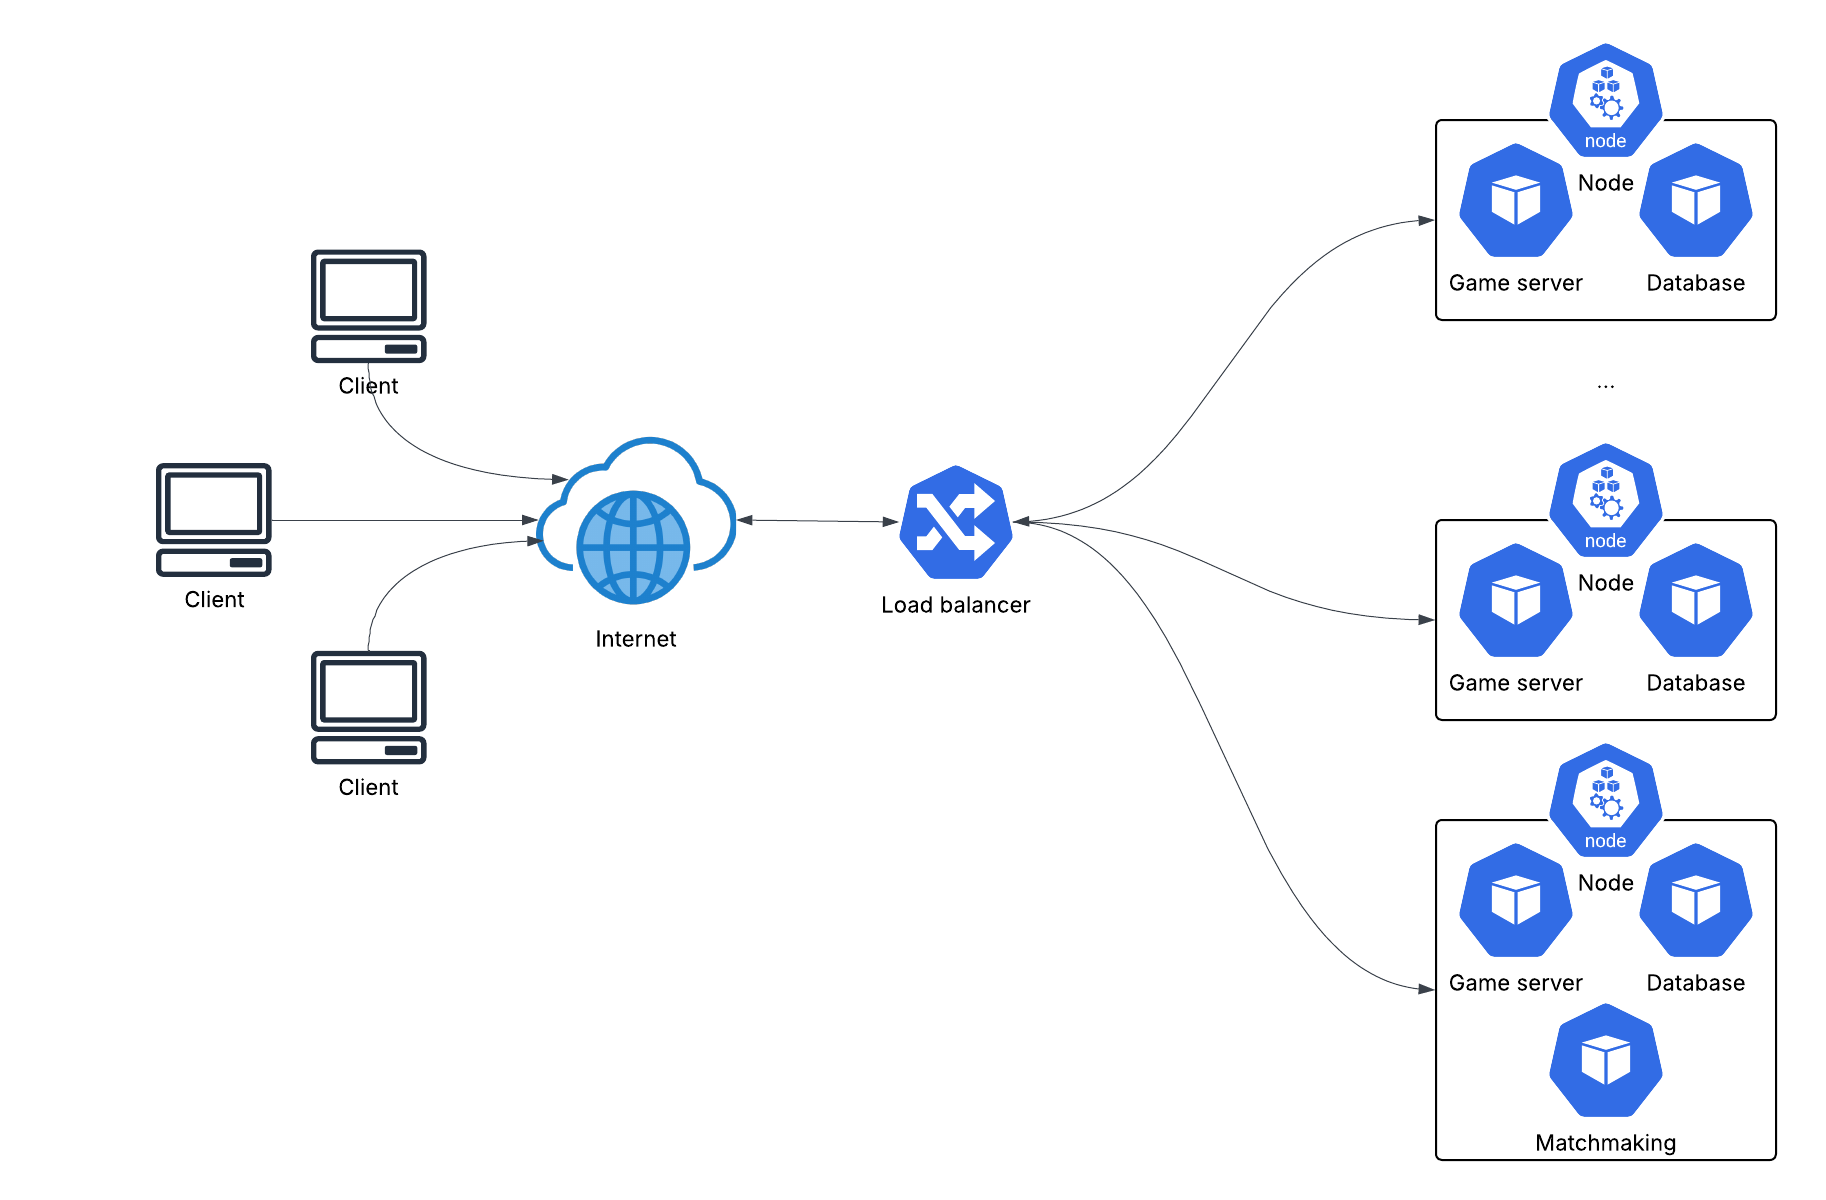
\includegraphics[width=0.75\textwidth]{figures/design/infrastructure.png}
  \caption{Deployment diagram of the system}
  \label{fig:infrastructure}
\end{figure}

\subsection{Modelling}\label{modelling}

\textbf{TODO: CLASS DIAGRAM: player, game with hand and cards}

\begin{itemize}
  \item which \textbf{domain entities} are there?
  %
  \begin{itemize}
    \item e.g.~\emph{users}, \emph{products}, \emph{orders}, \emph{etc.}
  \end{itemize}
  \textbf{Answer: } all the entities in model: player=user, game, hand, card. WebSocketHub
  
  \item how do \emph{domain entities} \textbf{map to/used by} \emph{infrastructural components}?
  %
  \begin{itemize}
    \item e.g.~state of a video game on central server, while inputs/representations on clients
    \item e.g.~where to store messages in an IM app? for how long?
  \end{itemize}
  \textbf{Answer: } state of a video game on database (server is stateless), while inputs/representations on clients.
  matchmaking service scans queue and creates game entities on the database and the game server alerts clients of the new game.

  \item which \textbf{domain events} are there?
  %
  \begin{itemize}
    \item e.g.~\emph{user registered}, \emph{product added to cart}, \emph{order placed}, \emph{etc.}
  \end{itemize}
  \textbf{Answer: } almost everything in the functional requirements. user registered, logged in, joined the queue
  left the queue, join a game, quit game, play again, play a card, choose a trump suit, player reconnection, game ended.
  
  \item which sorts of \textbf{messages} are exchanged?
  %
  \begin{itemize}
    \item e.g.~\emph{commands}, \emph{events}, \emph{queries}, \emph{etc.}
  \end{itemize}
  \textbf{Answer: } almost all domain events trigger messages, because everything has to be communicated to the clients.
  different queries to the database\ldots.

  \item what information does the \textbf{state} of the system comprehend
  %
  \begin{itemize}
    \item e.g.~\emph{users' data}, \emph{products' data}, \emph{orders' data}, \emph{etc.}
  \end{itemize}
  \textbf{Answer: } WebSocketHub holds information about the state of the connection and the client's identity.
  Only the database holds the state of the ongoing games, the matchmaking queue and the users' credentials.
\end{itemize}

\subsection{Interaction}\label{interaction}

\textbf{TODO: SEQUENCE DIAGRAM of matchmaking + timeout concurrent, playing a card}

\begin{itemize}
  \item how do components \emph{communicate}? \emph{when}? \emph{what}?
  \item \emph{which} \textbf{interaction patterns} do they enact?
\end{itemize}
\textbf{Answer: }the microservices communicate with the database through queries. Whereas the clients and the game server
communicat throughs WebSockets. Different message types are used to communicate client's intention and to update the client's game state.

\subsection{Behaviour}\label{behaviour}

\begin{itemize}
  \item how does \emph{each} component \textbf{behave} individually (e.g.~in \emph{response} to \emph{events} or messages)?
  \begin{itemize}
    \item some components may be \emph{stateful}, others \emph{stateless}
  \end{itemize}

  \item which components are in charge of updating the \textbf{state} of the system? \emph{when}? \emph{how}?
\end{itemize}
\textbf{Answer: }game server, martchamking and timeout are stateless, database is stateful.
database and clients change the state of the system: for instance clients make a move and the game state changes or matchmaking creates a game.

\subsection{Data and Consistency Issues}\label{data-and-consistency-issues}

\begin{itemize}
  \item Is there any data that needs to be stored?
  %
  \begin{itemize}
    \item \emph{what} data? \emph{where}? \emph{why}?
  \end{itemize}
  \textbf{Answer: }game state on database to store ongoing games. data is registered as key-value
  
  \item how should \emph{persistent data} be \textbf{stored}?
  %
  \begin{itemize}
    \item e.g.~relations, documents, key-value, graph, etc.
    \item why?
  \end{itemize}
  \textbf{Answer: } as key-value.
  
  \item Which components perform queries on the database?
  %
  \begin{itemize}
    \item \emph{when}? \emph{which} queries? \emph{why}?
    \item concurrent read? concurrent write? why?
  \end{itemize}
  \textbf{Answer: } game server and microservices. Which queries, how many, when? explain.
  
  \item Is there any data that needs to be shared between components?
  %
  \begin{itemize}
    \item \emph{why}? \emph{what} data?
  \end{itemize}
  \textbf{Answer: } yes the game state is shared throguht the DB
\end{itemize}

\subsection{Fault-Tolerance}\label{fault-tolerance}

\begin{itemize}
  \item Is there any form of data \textbf{replication} / federation / sharing?
  %
  \begin{itemize}
    \item \emph{why}? \emph{how} does it work?
  \end{itemize}
  \textbf{Answer: } yes, it is what we do with Kubernetes replication.
  
  \item Is there any \textbf{heart-beating}, \textbf{timeout}, \textbf{retry mechanism}?
  %
  \begin{itemize}
    \item \emph{why}? \emph{among} which components? \emph{how} does it work?
  \end{itemize}
  \textbf{Answer: } yes, it is to be integrated with the database client connection and kubernetes liveness.
  
  \item Is there any form of \textbf{error handling}?
  %
  \begin{itemize}
    \item \emph{what} happens when a component fails? \emph{why}? \emph{how}?
  \end{itemize}
  \textbf{Answer: } it panics and is recreated.
\end{itemize}

\subsection{Availability}\label{availability}

\begin{itemize}
  \item Is there any \textbf{caching} mechanism?
  %
  \begin{itemize}
    \item \emph{where}? \emph{why}?
  \end{itemize}
  \textbf{Answer: } No
  
  \item Is there any form of \textbf{load balancing}?
  %
  \begin{itemize}
    \item \emph{where}? \emph{why}?
  \end{itemize}
  \textbf{Answer: } Yes, Kubernetes

  \item In case of \textbf{network partitioning}, how does the system behave?
  %
  \begin{itemize}
    \item \emph{why}? \emph{how}?
  \end{itemize}
\end{itemize}
\textbf{Answer: } The state is mantained on the database and the users can recconect to another node automatically.
Game state is consistent when a partition from the user's side happens.

\subsection{Security}\label{security}

\begin{itemize}
  \item Is there any form of \textbf{authentication}?
  %
  \begin{itemize}
    \item \emph{where}? \emph{why}?
  \end{itemize}

  \item Is there any form of \textbf{authorization}?
  %
  \begin{itemize}
    \item which sort of \emph{access control}?
    \item which sorts of users / \emph{roles}? which \emph{access rights}?
  \end{itemize}

  \item Are \textbf{cryptographic schemas} being used?
  %
  \begin{itemize}
    \item e.g.~token verification,
    \item e.g.~data encryption, etc.
  \end{itemize}
\end{itemize}

\section{Implementation}\label{implementation}

Please report here all the implementation (technology-dependent) choices you made while implementing your design.

\begin{quote}
  If you run out of time for this project, you may consider leaving some aspect unimplemented, 
  and simply discuss how you would have implemented them.
  %
  In this case, better would be to discuss unimplemented features in \cref{future-works}.
\end{quote}

\begin{itemize}
  \item which \textbf{network protocols} to use?
  %
  \begin{itemize}
    \item e.g.~UDP, TCP, HTTP, WebSockets, gRPC, XMPP, AMQP, MQTT, etc.
  \end{itemize}

  \textbf{Answer:} we used HTTPS and WebSockets for delivering the web page
  and communicating the updates to the clients in a persistent way. 
  
  \item how should \emph{in-transit data} be \textbf{represented}?
  %
  \begin{itemize}
    \item e.g.~JSON, XML, YAML, Protocol Buffers, etc.
  \end{itemize}
  \textbf{Answer:} We used JSON for the messages to deliver updates
  and for the clients to send their moves.
  
  \item how should \emph{databases} be \textbf{queried}?
  %
  \begin{itemize}
    \item e.g.~SQL, NoSQL, etc.
  \end{itemize}
  \textbf{Answer:} NoSQL in particular queries to Etcd key-value storage.
  
  \item how should components be \emph{authenticated}?
  %
  \begin{itemize}
    \item e.g.~OAuth, JWT, etc.
  \end{itemize}
  \textbf{Answer:} the clients are authenticated throught classic password
  hashing comparing, also adding salt to enhance security. The password
  exchange security is backed by the TLS protocol implemented in the cluster.
\end{itemize}

\subsection{Technological details}\label{technological-details}

\begin{itemize}
  \item any particular \emph{framework} / \emph{technology} being exploited goes here
\end{itemize}

For the front-end we used React, as mentioned in the requirements, so that
the front-end updates on a state change.

\section{Validation}\label{validation}

\subsection{Automatic Testing}\label{automatic-testing}


\subsubsection*{Unit testing}

\subsubsection*{End-to-end testing}
End-to-end testing is performed throught Grafana K6, a framework that allows the automation
of load, performance and stress tests. Testing behaviour, users, iterations and checks are 
defined in JavaScript files and can be run with the K6 CLI.

All the tests simulate parallel users, open WebSocket connections and send messages to the server,
in particular:
\begin{itemize}
  \item \texttt{newMatch\_test.js} tests the user's registration, login and matchmaking process,
    verifying that the game is created.
  \item \texttt{match\_test.js} tests the whole game flow, from registering to playing cards.
    The users are instructed to play a card coherent to the table's state, otherwise a random card.
  \item \texttt{failedLogin\_test.js} simulates users trying to login without registering first.
    This ensures that the systems correctly handles unauthorized access.
  \item \texttt{wrongMessages\_test.js} simulates the users sending wrong messages without being logged in 
    to the server such as playing a card or choosing a trump.
    This check thats the server correctly verifies the identity of the connection before processing a message.
\end{itemize}

Tests are performed in the production environment (the Kubernetes cluster), so to run them 
the user needs to:
\begin{enumerate}
  \item install K6 from the \href{https://grafana.com/docs/k6/latest/set-up/install-k6/#install-k6}{official documentation}
  \item clone the \href{https://github.com/juturbo/MarafoNet}{project's repository}
  \item follow the instructions at the Section~\ref{deployment} to deploy the system
\end{enumerate}
Finally, the afromentioned tests can be run with the following command:
\begin{lstlisting}[language=bash]
  k6 run test_file.js
\end{lstlisting}

\begin{itemize}
  \item how were individual components \textbf{\emph{unit}-test}ed?
  Unit tests were performend on:
  \begin{itemize}
    \item DB querying components to validate the correct querying, and the connection itself
    \item the Model to validate the game logic, corner cases and point system
    \item the message service to check the correct message types
  \end{itemize}

  to test these you command \texttt{make test}.
  
  \item how to \textbf{\emph{end-to-end}-test} the system?
  %
  \begin{itemize}
    \item e.g.~production vs.~test environment
  \end{itemize}
  Testing end-to-end is automated throught Grafana K6 automatic testing
  in which the K6 framework simulates users registering, logging in and
  playing a few cards.
  To run this test one must first deploy the cluster by following the
  instruction at the Section~\ref{deployment} and then run:
  \texttt{k6 run register\_test.js}.

  \item for each test specify:
  %
  \begin{itemize}
    \item rationale of individual tests
    \item how were the test automated
    \item how to run them
    \item which requirement they are testing, if any
  \end{itemize}
\end{itemize}

\begin{quote}
recall that \emph{deployment} \textbf{automation} is commonly used to \emph{test} the system in \emph{production-like} environment
\end{quote}

\begin{quote}
recall to test corner cases (crashes, errors, etc.)
\end{quote}

\subsection{Acceptance test}\label{acceptance-test}

\begin{itemize}
  \item did you perform any \emph{manual} testing?
  %
  \begin{itemize}
    \item what did you test?
    \item why wasn't it automatic?
  \end{itemize}
\end{itemize}

\section{Deployment}\label{deployment}
\subsection{Image building}
Container images for the game server and the matchmaking service are built from
source code by a GitHub Action Workflow; the same action releases the images to
the project's repository.

The images are then publicly available and can be pulled directly from GHCR
to be deployed on Kubernetes.
\subsection{Manifests}
Manifests in the \texttt{deployment/kubernetes} directory specify the deployment's
characteristics such as the replica count for each pod, where the pods should be placed 
and which ports to open.

The \texttt{marafonet-deployment.yaml} file defines an environment variable containing
the Etcd pods' addresses and a rule so that the pods from this deployment are scheduled
in different nodes to ensure availability.

The \texttt{marafonet-hpa.yaml} creates an Horizonal Pod Autoscaler so that the replica
count of the Game Server's pods can change dinamically according to processor and memory
usage.

Other files define the Etcd cluster and the Ingress, a component that acts both as load 
balancer and TLS terminator.
\subsection{Requirements}\label{deployment-requirements}
To deploy the application the following software must be installed on the target machine:
\begin{itemize}
  \item \href{https://docs.docker.com/engine/install}{Docker} (depending on the operating system, it may be necessary to install Docker Desktop)
  \item \href{https://minikube.sigs.k8s.io/docs/start}{minikube}
  \item \href{https://kubernetes.io/docs/tasks/tools/#kubectl}{kubectl}
\end{itemize}
After successful installation the user can proceed to the next section.
%
\subsection{Deployment instructions}
First, the user needs to start the Kubernetes cluster throught \texttt{minikube}:
\begin{lstlisting}[language=bash]
  ~$ minikube start --nodes 3 --driver=docker -p marafonet-cluster
\end{lstlisting}
this will create a local cluster on Docker containers.

Then, the user needs to enable the Ingress controller on the cluster with the following command:
\begin{lstlisting}[language=bash]
  ~$ minikube addons enable ingress -p marafonet-cluster
	~$ kubectl wait --namespace ingress-nginx 
  \ --for=condition=ready pod 
  \ --selector=app.kubernetes.io/component=controller
  \ --timeout=120s
\end{lstlisting}

\textbf{TODO: ADD SCREENSHOTS OF THE COMMANDS' OUTPUT}

Once the cluster is running, the user needs to create TLS certificates and the
relative Kubernetes secret that will be used for HTTPS connection, to do this
\texttt{OpenSSL} can be used. In a temporary directory, run:
\begin{lstlisting}[language=bash]
  	~$ openssl req -x509 -newkey rsa:4096 -sha256 -nodes -keyout \
    ./tls.key \ 
    -out ./tls.crt \
    -subj "/CN=localhost" -days 365
\end{lstlisting}
Then the secret can be created with the following command:
\begin{lstlisting}[language=bash]
kubectl create secret tls marafonet-tls --key ./tls.key --cert ./tls.crt
\end{lstlisting}

All the Kubernetes' resources are grouped inside a \texttt{kustomize.yaml} file
that can be used to deploy the system throguht \texttt{kubectl apply} command.
\begin{lstlisting}[language=bash]
  ~$ kubectl apply -k github.com/juturbo/marafonet/deployment/kubernetes
\end{lstlisting}
the command should output the following:
\begin{figure}[H]
  \centering
  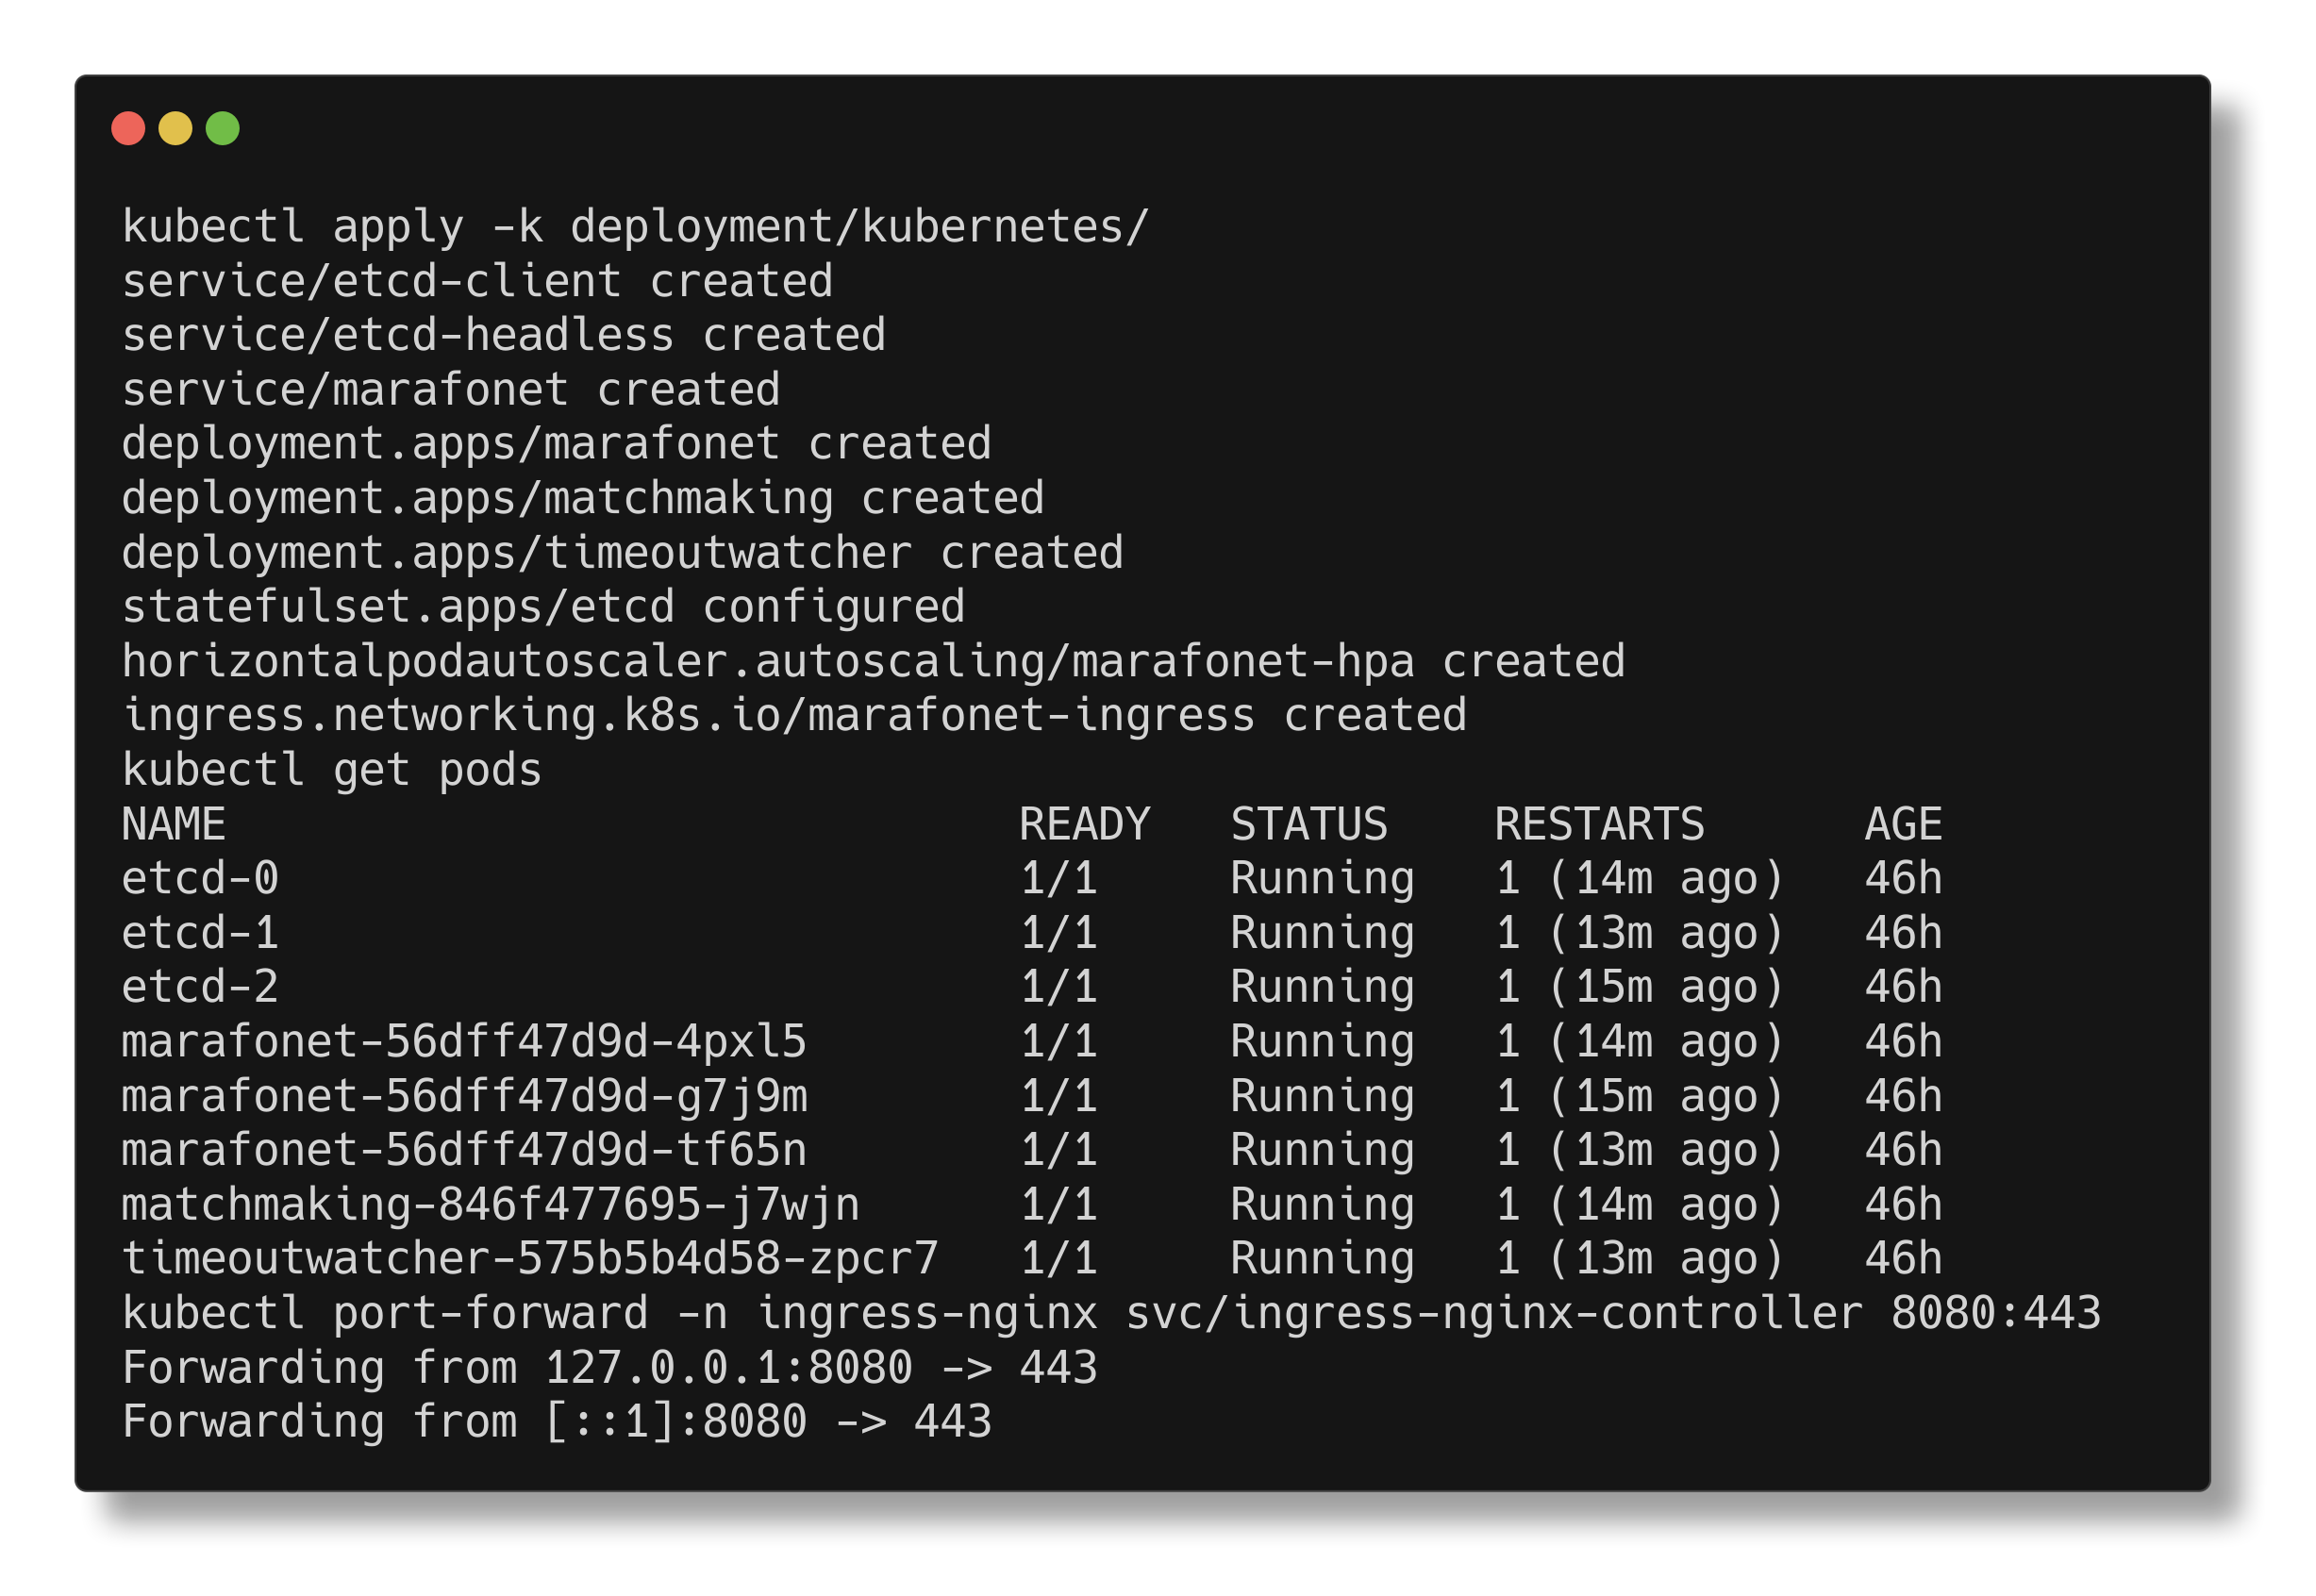
\includegraphics[width=0.75\textwidth]{figures/deployment/deployment-instructions.png}
  \caption{Deployment command output}
  \label{fig:instructions-output}
\end{figure}

\section{User Guide}\label{user-guide}

\begin{itemize}
  \item how to use your software?
  %
  \begin{itemize}
    \item provide instructions
    \item provide expected outcomes
    \item provide screenshots if possible
  \end{itemize}
\end{itemize}

\section{Self-evaluation}\label{self-evaluation}

\begin{itemize}
  \item An individual section is required for each member of the group
  \item Each member must self-evaluate their work, listing the strengths and weaknesses of the product
  \item Each member must describe their role within the group as objectively as possible.
\end{itemize}

It should be noted that each student is only responsible for their own section.

\section{Future works}\label{future-works}

Discuss possible future works, improvements, extensions, optimizations, etc.

Also discuss here any unimplemented feature, and how you would have implemented it.

%\bibliographystyle{plain}
%bibliography{references}

\end{document}
